\graphicspath{{Ch1_Theory/figures/}}

\chapter{Theoretical Background}

\nomenclature[A]{SM}{The \textbf{S}tandard \textbf{M}odel of Particle Physics}
\nomenclature[A]{QFT}{\textbf{Q}uantum \textbf{F}ield \textbf{T}heory}

The Standard Model (SM) of particle physics is the most successful theory in the history of human scientific endeavour\footnote{According to physicists, of course.}.
It provides a unified framework describing the electromagnetic, weak, and strong interactions along with all known particles that participate in those interactions.
The fundamental objects in the SM description are fields defined at all points in spacetime.
The SM fields fall into four main categories:
\begin{enumerate}
    \itemsep0em 
    \item Fermionic fields, $\Psi$, describing ``matter'': quarks and leptons;
    \item Electroweak spin-1 boson fields,
        \begin{itemize}
            \item $W_1, W_2, W_3, B$: before symmetry breaking.
            \item $W^+, W^-, Z^0, \gamma$: after symmetry breaking.
        \end{itemize}
    \item Gluon fields, $G_a$;
    \item The Higgs field, $\Phi$.
\end{enumerate}

The dynamics of these fields and their interactions are predicted via the mathematical framework of Quantum Field Theory (QFT).
In this chapter a compact but complete overview of the mathematical framework of the Standard Model is given.

\section{Minkowski Spacetime}
\newcommand{\MinkSpace}{\ensuremath{\mathbb{R}^{3,1}}\xspace}
The arena in which all particles are embedded in the Standard Model is the pseudo-Riemannian manifold \MinkSpace, otherwise known as \textit{Minkowski space} or \textit{Minkowski spacetime}.
The spacetime location of any \textit{event}, such as a particle collision or decay, can be encoded as a vector with four elements: $p = (ct, x, y, z)$, where $c$ is the \textbf{speed of light}.
From this point onwards the common particle physics convention of setting $c = 1$ will be used\footnote{At the end of any calculation, dimensional analysis can be used to restore the true value of c to the result.}.
The distinction between normal four-dimensional Euclidean space $\mathbb{R}^4$ and Minkowski space \MinkSpace is necessary due to the discoveries of Hendrik Lorentz and Albert Einstein culminating in the special\footnote{General relativity, which accounts for gravity by including the possibility of curvature into spacetime, is not (yet) part of the Standard Model. This is, to put it mildly, an area of active interest for many theorists.} theory of relativity, which proceeds from two postulates:
\begin{enumerate}
    \item The laws of physics are invariant in all inertial (non-accelerating) frames of reference.
    \item The speed of light in a vacuum is the same for all observers, \textit{regardless} of the motion of the light source or observer.
\end{enumerate}

The second postulate complicates the notion of transforming between frames of reference, which must be done carefully to ensure the validity of the first postulate.
To address this Minkowski space is equipped with a metric $\eta$ often referred to as the \textit{Minkowski metric} which is used to compute the distance between two spacetime events in a manner slightly different than traditional Euclidean space:
\begin{equation}
\mu =
\begin{bmatrix} 
1 & 0 & 0 & 0\\
0 & -1 & 0 & 0\\
0 & 0 & -1 & 0\\
0 & 0 & 0 & -1\\
\end{bmatrix}
\end{equation}
which can be used to define a bilinear form over arbitrary pairs of spacetime points $p_1$ and $p_2$,
\begin{equation}
p_1 \cdot p_2 \equiv p_1^T\; \eta\; p_2 = t_1t_2 - x_1x_2 - y_1y_2 - z_1z_2
\end{equation}

The \textbf{spacetime interval} $\Delta s$ between any two events in the same inertial frame of reference, $p_1 \equiv (t_1, x_1, y_1, z_1)$ and $p_2 \equiv (t_2, x_2, y_2, z_2)$, can be expressed in terms of this bilinear form:
\begin{align*}
    \Delta s(p_1, p_2) &\equiv \sqrt{(p_1-p_2) \cdot (p_1-p_2)} \\
    &= \sqrt{
        (t_1-t_2)^2 - (x_1-x_2)^2 - (y_1 - y_2)^2 - (z_1 - z_2)^2
    }
\end{align*}
With some simple algebra it follows directly from the second postulate of special relativity that $\Delta s$ must be invariant under changes of inertial reference frame. In other words, for two spacetime points in one inertial frame of reference ($p_1$, $p_2$) and their representation in a different inertial frame of reference ($p_1'$, $p_2'$), it must hold that $\Delta s(p_1, p_2) = \Delta s(p_1', p_2')$ for \textit{any} arbitrary pair of inertial reference frames.

\begin{tcolorbox}
\paragraph{Einstein Notation} 
In order to simplify expressions, summation over indices is often abbreviated in particle physics: $x_i y^i \equiv \sum_i x_i y^i$.
For the case of four-vectors from Minkowski spacetime the summation notation implicitly carries the application of the Minkowski metric:
$x_\mu y^\mu \equiv x \cdot y \equiv \sum_{\mu\nu} \eta_{\mu\nu} x^\mu y^\nu$.
The distinction between lower (covariant) and upper (contravariant) indices is mathematically important but not necessary for our purposes here.
\end{tcolorbox}

A very good question to ask at this point is: what types of transformations are allowed between inertial frames of reference?
To state this question mathematically, if we write an arbitrary transformation as $p' = \Lambda p$, what are the range of possibilities for $\Lambda$ which preserve the spacetime interval $\Delta s$?
Intuitively we may have an idea of what these transformations will look like, but these must be mathematically codified.
This is best accomplished via the mathematical framework of \textbf{group theory}.

Developing the language and concepts of group theory is beyond the scope of this dissertation, but it can be shown that the $\Lambda$ objects mentioned above are the members of the \textbf{Poincar\'{e} group}, which is
the \textit{isometry group} of Minkowski space, i.e. the set of all bijective $\Delta s$-preserving maps from \MinkSpace to \MinkSpace.
These transformations fall into three categories:
\begin{itemize}
\itemsep0em 
\item \textbf{translations} in time and/or space
\item \textbf{rotations/reflections} in three-dimensional space
\item \textbf{boosts} or constant shifts in velocity
\end{itemize}
These separate categories may be combined freely, which means the Poincar\'{e} group has ten dimensions: four for translations, three for rotations/reflections, and three for boosts.
Any mathematical framework for making predictions about particle physics must be, at minimum, invariant with respect to these types of transformations.

\section{Fields and the Action Principle}
The foundation for making physical predictions about fundamental particle physics is the \textbf{action principle}, which provides a mathematical framework \cite{Feynman:1942us} for computing the probability amplitude for a system of particles to evolve from some initial quantum state $\ket{\Psi_I}$ at time $t=0$ to a state $\ket{\Psi_F}$ at time $t=T$:
\begin{align}
    \bra{\Psi_F} e^{-i\hat{H}T} \ket{\Psi_I} &= \int_{\Psi_I}^{\Psi_F} \mathcal{D}_{\Psi}(t)\; \exp \left\{ \frac{i}{\hbar} S \right\}, \label{eq:path_integral} \\
    S &= \int_0^T dt\; L \left( \left\{ \Psi \right\}, \left\{ \partial_\mu \Psi \right\} \right) \nonumber
\end{align}
where $\hat{H}$ is the Hamiltonian operator\footnote{It may make intuitive sense to think of fields as smooth functions of spacetime. However, in actuality they are \textit{operators} acting on the state space of the SM, here represented by $\ket{\phi_I}, \ket{\phi_F}$. The details and importance of this are beyond the scope of this dissertation.} corresponding to the total energy of the system of particles, $S$ is the \textbf{action}, $L$ is the \textbf{Lagrangian} which is an expression built from all the relevant particle fields $\left\{ \Psi \right\}$ as well as their derivatives with respect to spacetime $\left\{ \partial_\mu \Psi \right\}$, and $\mathcal{D}_{\Psi}(t)$ is the differential element for integrating over \textit{all possible} system trajectories the system could take from $\ket{\Psi_I}$ to $\ket{\Psi_F}$.
Thus the probability amplitude is computed as a \textit{weighted sum} over all possible system trajectories, where the weight is $\exp \left\{ \frac{i}{\hbar} S \right\}$.
Once the Lagrangian is defined, arriving at the resulting physical predictions is only\footnote{In practice this is \textit{extremely} difficult and time consuming.} a matter of carrying out the calculations to compute the relevant probability amplitudes.

One important job of the theoretical particle physicist is to construct a Lagrangian in such a way as to match and/or predict experimental results.
In order to construct a Lagrangian one must put constraints on what sort of fields are allowed to enter into the expression and how those fields can be used in the expression.
Following from work of Eugene Wigner~\cite{Bargmann:1948ck}, all the mathematical structures (fields) used to describe particles in the Standard Model must be part of a positive-energy irreducible unitary representation of the Poincar\'{e} group.
This subset of the Poincar\'{e} group representations can be indexed by two properties possessed by every fundamental particle: mass\footnote{The mass of a particle can of course be zero.} (a non-negative number) and spin (an integer or half integer such as 0, 1/2, 1, 3/2, \dots).
The Lagrangian encodes the laws of physics for a particular theory, and we know that the laws of physics must be invariant under Poincar\'{e} transformations as discussed in the previous section.
Therefore the Lagrangian itself must be invariant under these transformations.
This severely restricts the types of terms that can be allowed in the Lagrangian.

Particles in the SM have \textit{internal} properties which must be encoded in the Lagrangian as well.
This means that the symmetry group under which the Lagrangian is invariant must actually be defined by the \textit{direct product} of multiple groups, with some encapsulating global properties of spacetime itself (global symmetries), and others encoding the internal degrees of freedom of the particles embedded in this spacetime (local symmetries).
There are three predominant local symmetries in the SM and each one is associated with special properties of a particular subset of SM particles.
These local symmetries arise through the electromagnetic force associated with the $U(1)$ group, the weak force associated with the $SU(2)$ group, and the strong force associated with the $SU(3)$ group.

\section{Gauge Invariance}
Local symmetries lead to presence force-carrying particles in the Lagrangian through a requirement called \textbf{gauge invariance}.
A \textbf{gauge} is a particular choice of values for any redundant degrees of freedom underlying the mathematical formalism of a local symmetry group.
A \textbf{gauge transformation} is a simultaneous change in these redundant degrees of freedom.
A \textbf{gauge theory} is a physical model based on a Lagrangian to which gauge transformations can be applied, but with the important caveat that the \textit{physical predictions remain the same} regardless of which gauge is used.
The motivation for the concepts underlying gauge theory are largely analogous to the intuitive notion that physical predictions in classical mechanics remain the same regardless of which inertial frame of reference is used to perform the calculation.
% mention t'hooft gauge, epsilon gauge, etc

For example, consider a single particle quantum mechanical system with time-independent Hamiltonian $H$ and energy eigenstates $\ket{n}$.
To make a physical prediction for the probability for some general solution to the Schroedinger equation $\left( \ket{\phi} = \sum_n c_n e^{-iE_nt / \hbar} \ket{n} \right)$ to be observed in eigenstate $\ket{n}$, one calculates the transition probability $\left| \bra{n} H \ket{\phi} \right|^2$.
However, if one were to transform all the eigenstates by $\ket{n} \rightarrow e^{i\theta_n} \ket{n}$, the probability would not change, even though you have ostensibly changed the eigenstates.
In this case the \textit{gauge} is a choice of values for $\theta_n$ and a \textit{gauge transformation} would entail a change $\theta_n \rightarrow \theta_n + \Delta\theta_n$ for some arbitrary set of $\Delta\theta_n$.

In this sense, while the computations are performed in $H$, the physical states themselves actually reside in $P(H)$, the \textit{projective} Hilbert space.
This projective Hilbert space contains a set of all equivalence classes of states where $\ket{n} \sim e^{i\theta_n}\ket{n}$, for any $\theta_n$.
This should not be taken to mean that the redundant degrees of freedom in a gauge theory, like the complex phase factor above, are without meaning at all. 
While they are not themselves measurable, their presence in the theory has measurable \textit{consequences}.
For example, the presence of complex phase factors in QM is what leads to the famous double slit and Ahranov-Bohm effects.
These consequences arise from the \textit{difference} in phase factors between states that naturally arise throughout the calculation, but do not depend on the initial choices of $\theta_n$. This is what is meant by the phrase \textit{redundant degrees of freedom}.

In short, the necessity for gauge invariance is that the mathematical/computational framework of a theory may have its \textit{own} internal machinery which contributes to the result, but has some arbitrary aspects which do not alter the final physical prediction.
Once we include any purely computational degrees of freedom in our theory we must demand that our theory is invariant with respect to the most general possible change in them that does not alter the physical prediction.
In the words of Murray Gell-Mann, ``Everything not forbidden is compulsory'', a sentiment at the heart of modern physics.
To state it another way: any arbitrary element of a theory must be treated as \textit{maximally} arbitrary in order to preserve its integrity.

One aspect left out of the simple quantum mechanics example above is the notion of a gauge which varies with respect to spacetime itself.
To begin, imagine you have two $n$-dimensional vectors $A$ and $B$ in familiar Euclidean space $R^n$. In order to compare vector $A$ to vector $B$, vector $A$ must be \textit{transported} so that the tails of $A$ and $B$ are located at the same point.
Furthermore, this transport must be done while keeping $A$ \textit{parallel} to its original direction in order to preserve geometric information such as the relative angle betwen $A$ and $B$.
This process is precisely the same as the way in which you would bring two everyday objects together to compare them in the real world.
The reason this works and is intuitive is that $R^n$ is a flat space and maintaining the orientation and relevant properties of normal objects requires no special care to preserve when moving them around.

\newcommand{\conn}{ \ensuremath{ \boldsymbol{\mathcal{A}} } }
However, if one is operating on fields with a spacetime varying gauge corresponding to some local symmetry group, the notion of \textbf{parallel transport} must be refined in order to compare fields at separate points in spacetime.
Consider an extension of the gauge invariance example from quantum mechanics above to a field with a spacetime varying gauge which can be arbitrarily transformed without altering the physical predictions: $\psi \rightarrow e^{i\alpha(x)} \psi$.
This gauge $\alpha(x)$ is \textit{non-physical} in the same manner as the phase factors $\theta_n$ in the previous example.
Due to the freedom of gauge choice, in order to compare the field values as different points of spacetime what is needed then is not just a measure of the change in a field, but a measure of the change in a field \textit{relative} to the change that occurs purely due to the variations in the gauge itself.
The \textbf{gauge covariant derivative} $D_\mu(x) \equiv \partial_\mu + \conn_\mu(x)$ achieves precisely this.
The extra spacetime-dependent term $\conn_\mu(x)$ that addresses the effect of the spacetime-varying gauge of the local symmetry group is known as the \textbf{connection}.
Somewhat mysteriously the \textit{force-carrying} particles of the SM, such as photons, manifest through this connection.

% A simple pedagogical example is useful here. Consider the following Lagrangian density\footnote{The Lagrangian is often written as an integral over spacetime of the Lagrangian density: $L = \int d^4x \mathcal{L}$} for a set of $n$ non-interacting real-valued scalar fields with equal masses $m$:
% \begin{equation}
% \mathcal{L} = \sum_{i=1}^{n} \left[ \frac{1}{2} \partial_\mu \varphi_i \partial^\mu \varphi_i - \frac{1}{2} m^2 \varphi_i^2 \right].
% \end{equation}
% which is clearly invariant under Poincar\'{e} transformations.
% In order to begin exploring the relationship between the separate $\varphi_i$ fields we may write them as a self-contained vector $\Phi = (\varphi_1, \varphi_2, \varphi_3, \dots, \varphi_n)$.
% This allows us to rewrite the Lagrangian:
% \begin{equation}
% \mathcal{L} = \frac{1}{2} (\partial_\mu \Phi)^T \partial_\mu \Phi - \frac{1}{2} m^2 \Phi^T \Phi
% \end{equation}
% %TODO: show einstein notation somewhere and mention what sort of terms are invariant under poincare transformations
% 
% One additional symmetry constraint we can impose upon the Lagrangian is a global symmetry under the orthogonal group\footnote{The specific nature of the $O(n)$ group is not important here, since we only seek to demonstrate the process of imposing additional symmetry constraints upon a Lagrangian.} $O(n)$ transformations applied to $\Phi$, which are represented by constant $n$-dimensional matrices $G$ in this representation.
% The principle property of these matrices is that $G^T G = G G^T = I$, where $I$ is the identity matrix.
% In fact the Lagrangian is already invariant under these global transformations:
% \begin{align}
% \Phi &\rightarrow G\Phi \\
% \partial_\mu \Phi &\rightarrow \partial_\mu(G\Phi) = G \partial_\mu \Phi \\
% \mathcal{L} &\rightarrow \frac{1}{2} (G \partial_\mu \Phi)^T (G \partial_\mu \Phi) - \frac{1}{2} m^2 (G \Phi)^T (G \Phi) \\
% &= \frac{1}{2} (\partial_\mu \Phi)^T\; (G^TG)\; \partial_\mu \Phi - \frac{1}{2} m^2 \Phi^T (G^T G) \Phi \\
% &= \frac{1}{2} (\partial_\mu \Phi)^T (\partial_\mu \Phi) - \frac{1}{2} m^2 \Phi^T \Phi
% \end{align}
% 
% At this point we should generalize this symmetry to vary in a continuous manner with respect to spacetime ($G \rightarrow G(x)$) for the reasons given earlier in this section.
% The spacetime derivatives $\partial_\mu$ must now be extended to include a connection.
% We define the gauge covariant derivative as %TODO: reference original equation
% \begin{equation}
% D_\mu = \partial_\mu - igA_\mu(x)
% \end{equation}
% where the $-i$ is for mathematical convenience and the $g$ parameter is extracted to quantify separately the ``strength'' of the connection.
% By utilizing this form for $D_\mu$ and imposing local $O(n)$ invariance on the Lagrangian, a simple calculation shows that the gauge field $A_\mu$ \textit{must} transform as
% \begin{equation}
% A_\mu \rightarrow A_\mu' = G A_\mu G^{-1} - \frac{i}{g}(\partial_\mu G) G^{-1}.
% \end{equation}
% where the spacetime dependence $A\mu(x)$ and $G(x)$ has been omitted only for readability.

Groups which are continuously parameterized by some number of real-valued parameters are called \textit{Lie groups}, and all the local symmetry groups of the Standard Model fall into this category.
In the case of a quantum field theory with a local symmetry Lie group, the connection is an element of the corresponding Lie Algebra\footnote{A Lie Group $G$ and its Lie Algebra $\mathfrak{g}$ are related by an \textit{exponential map} which allows for any group element $X \in G$ to be written as $e^{it}$ for some linear combination $t$ of the elements of $\mathfrak{g}$.} $\mathfrak{g}$.
This means the connection can be written as a linear combination of the infinitesimal generators $T_a$ of the Lie algebra.
Thus $\conn_\mu$ can be expanded as $\conn_\mu \equiv A_\mu^a T_a$, where the different $A_\mu^a$ terms transform under the adjoint representation of the local symmetry group.
In physics it is common notational practice to define $D_\mu \equiv \partial_\mu - igA_\mu^aT_a$, where $g$ is a dimensionless \textit{coupling constant}.
The $A_\mu^a$ terms are referred to as \textit{connection coefficients}.
In fact these connection coefficients will turn out to be the fields for the ``force-carrying'' gauge bosons of the Standard Model.

\begin{tcolorbox}
\paragraph{Notation} Greek letters $\mu,\nu,\dots$ will be used to index Minkowski space, and alphabetic characters $a,b,\dots$ will be used to index the Lie algebra generator basis.
Einstein summation notation is assumed throughout.
\end{tcolorbox}

\section{Yang-Mills Theory}
With the covariant derivative we can construct the \textbf{curvature form} $F_{\mu\nu} \equiv \frac{1}{g} \comm{D_\mu}{D_\nu}$.
A simplified picture of the curvature is that it encodes the \textit{strength} and geometric properties of the gauge field $A_\mu$ at each point in spacetime.
For this reason, the curvature is usually referred to as the \textbf{field strength tensor} in physics and is always part of the Lagrangian.

The starting point for constructing the Standard Model is Yang-Mills gauge theory, which finds its fullest and most beautiful expression in the language of differential geometry.
In the case of the Standard Model, we can dispense with some of the abstract notions of differential geometry and restrict our attention to theories taking place in Minkowski Space.
The previous expression given for the curvature can be expanded as
\begin{align}
    F_{\mu\nu} &= \partial_\mu \conn_\nu - \partial_\nu \conn_\mu + ig\comm{\conn_\mu}{\conn_\nu}\\
    &= \partial_\mu A_\nu^aT_a - \partial_\nu A_\mu^aT_a + ig\comm{A_\mu^aT_a}{A_\nu^bT_b}\\
    \implies F_{\mu\nu}^a &= \partial_\mu A_\nu^a - \partial_\nu A_\mu^a + igf^a_{\ bc}A_\mu^bA_\nu^c
\end{align}
where $f^a_{bc} \equiv $ are the \textbf{structure constants} of the associated Lie algebra.
If the associated Lie group is \textit{abelian}, i.e. the generators commute, then the structure constants vanish.
This is the case for $U(1)$, the local symmetry group associated with electromagnetism.

In this system of notation, the \textbf{Yang-Mills Action} can be written
\newcommand{\YML}{ \ensuremath{ \mathcal{L}_{\mathrm{YM}} } }
\begin{align}
    S_{\mathrm{YM}} &= \int d^4x\ \YML\\
    \mathrm{where}\ \YML &= -\frac{1}{4} F_{\mu\nu}^a F^{\mu\nu}_a
\end{align}
which is both Poincar\'{e} and gauge invariant. It is important to recognize that two bilinear forms are involved in the above expression, one acting over the indicies of the Lie algebra for the local symmetry group and one over indices of Minkowski space.

A Yang-Mills theory can be expanded by embedding more fields into Minkowski space
\newcommand{\YM}{ \ensuremath{ \mathcal{L}_m\left( \left\{ \boldsymbol\Psi \right\}, \left\{ D_\mu \boldsymbol\Psi \right\} \right) }}
\begin{equation}
    \mathcal{L} = \YM + \YML
\end{equation}
where $\left\{ \boldsymbol\Psi \right\}$ is some set of new fields which transform under the fundamental representation of the internal symmetry group and, by virtue of $D_\mu$, couple to the force-carrying particle associated with the relevant local symmetry.
The new $\mathcal{L}_m$ term must be Poincar\'{e} and gauge invariant as well, which can be achieved by judicious use of bilinear covariants and substitution of the standard spacetime derivative $\partial_\mu$ with the covariant derivative $D_\mu$.

\section{The Standard Model}
The Standard Model of particle physics is a Yang Mills gauge theory with local symmetry group $SU(3) \otimes SU(2) \otimes U(1)$.
It describes the strong, weak, and electromagnetic interactions which occur via the exchange of the corresponding spin-1 gauge fields: eight massless gluons from $SU(3)$, three massive weak bosons ($W^\pm$, Z) from $SU(2)$ and one massless photon from $U(1)$.
The matter fields of the SM are given by a three-tiered family of leptons and quarks as shown in Figure~\ref{fig:sm_breakdown}.
Each family has identical properties other than the mass and \textit{flavour} quantum number of the corresponding particles, which denotes which of the three families the particle belongs to.

\begin{figure}[h]
   \centering
    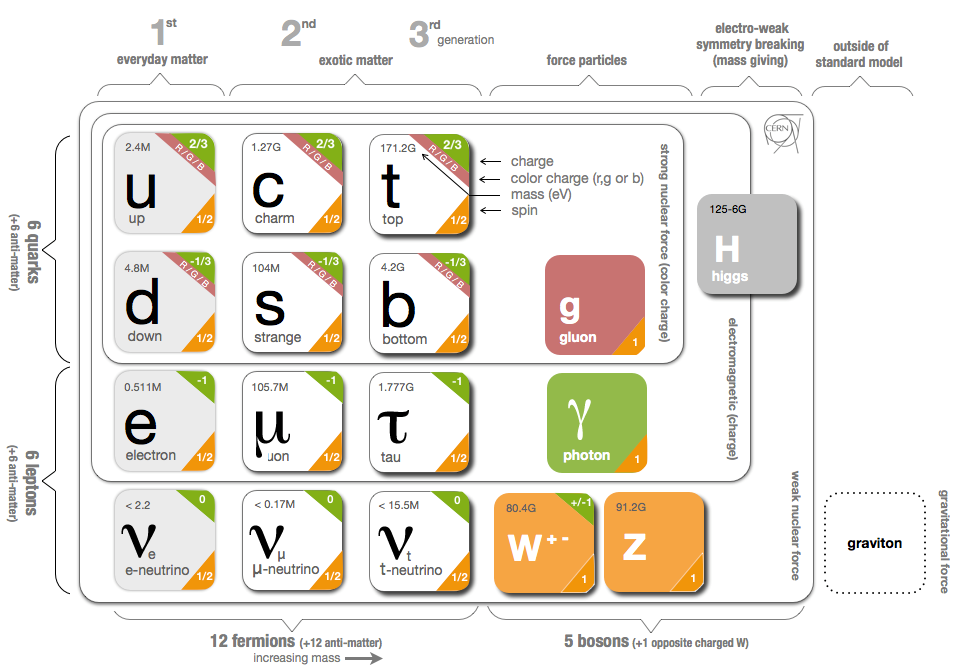
\includegraphics[width=\textwidth]{SMdiagram}
    \caption{Phenomenological breakdown of the Standard Model. © 2014 CERN}
	\label{fig:sm_breakdown}
\end{figure}

As mentioned previously all fields of the SM are constructed as positive-energy irreducible unitary representations of the Poincar\'{e} group.
The particular representations used in the SM are subtle, accounting for the peculiarities of the nature of the interactions involved such as quark/lepton flavor, color, chirality, and spin.
This results in significant complexity in the final representation, where for example the total fermionic field content of the SM has 96 complex-valued components.
For the purposes of this dissertation the focus will be on the overall structure of the SM as it relates to the observed interactions in nature, as opposed to the full mathematical details.

\subsection{Electroweak Interaction}
The combined $SU(2) \otimes U(1)$ component of the Standard Model is known as the Electroweak interaction and consists of the unification of two fundamental interactions in nature: \textit{electromagnetism} and the \textit{weak interaction}.

The Lagrangian density for the electroweak interaction is given by
\begin{align}
    \mathcal{L}_{\mathrm{EW}} &= \sum_{\Psi}  \bar{\Psi}  (i \gamma^\mu D_\mu) \Psi - \frac{1}{4} W_a^{\mu\nu} W^a_{\mu\nu} - \frac{1}{4} B^{\mu\nu}B_{\mu\nu} \\
    D_\mu &= \partial_\mu + i g T_a W_\mu^a + i \frac{g'}{2} B_\mu
    \label{eq:ew_deriv}
\end{align}
where $W^a_{\mu\nu}$ for $a \in (1,2,3)$ are field strength tensors for the local $SU(2)$ symmetry called \textbf{weak isospin}, $B^{\mu\nu}$ is the field strength tensor for the local $U(1)$ symmetry called \textbf{weak hypercharge}.
The fields $W_\mu^j$ and $B_\mu$ are the corresponding connections for weak isospin and hypercharge, with coupling constants factored out as $g$ and $g'$. Note that here we use the same base symbol ($W$ and $B$) for both the connection coefficients and field strength tensor, whereas previously we used separate symbols: $F_{\mu\nu}$ and $A_\mu$.
The generators of $SU(2)$ are given by $T_a$ and $Y$, respectively.
Due to the simplicity of the $U(1)$ group, $Y$ is simply a real number, whereas $T_a$ for $a \in (1,2,3)$ are the $2\times2$ Pauli matrices.
The $\Psi$ fields are the fermions which are represented as \textit{spinors} in the SM, which necessitates the use of the \textbf{gamma matrices} $\gamma^\mu$ to apply the covariant derivative $D_\mu$.

There are a number of subtle complicating factors hidden in the definition of $\mathcal{L}_{\mathrm{EW}}$.
The weak isospin symmetry is \textit{chiral} and only affects left-handed particles, where ``handedness'' depends on the orientation of the particle spin relative to its momentum\footnote{This is an oversimplification of \textit{chirality}, one of the more difficult aspects of the SM to understand.}.
Thus the $\Psi$ fields outlined above are a combination of $SU(2)$ doublets for the left-handed fermions and singlets for the right-handed fermions.
\begin{equation}
    \Psi = \begin{pmatrix}
           \nu_{l_i} \\
           l_i
         \end{pmatrix}_L,\;
         (l_i)_R,\;
    \begin{pmatrix}
           u_i \\
           d_i
        \end{pmatrix}_L,\;
        (u_i)_R,\; (d_i)_R
\end{equation}
where the index $i \in (1,2,3)$ runs over the three families of quarks ($u_i$, $d_i$), charged leptons ($l_i$) and neutrinos ($\nu_{l_i}$).
The left-handed doublet quark fields in $\Psi$ are not the same as the quark fields under the strong interaction, but rather a mixture of them, which are related by the Cabibbo-Kobayashi-Maskawa (CKM) matrix \cite{Kobayashi:1973fv, Cabibbo:1963yz}.

\subsection{Strong Interaction}
Quantum Chromodynamics (QCD) is the theory of the \textit{strong interaction} between quarks and gluons, which are the primary constituents of ordinary matter such a protons and neutrons, as well as less common hadrons such as the pion.
The analogue of electric charge from QED is \textit{color charge} in QCD, and the corresponding force-carrying particle is the gluon.
The local symmetry group for QCD is SU(3), leading to the following Lagrangian:
\begin{align}
    \mathcal{L}_{\mathrm{QCD}} &= \sum_{q}  \bar{\Psi}_q  (i \gamma^\mu D_\mu) \Psi_q - \frac{1}{4} G_a^{\mu\nu} G^a_{\mu\nu} \\
    D_\mu &= \partial_\mu - i g_s G_\mu^a T_a
\end{align}
where $G_a^{\mu\nu}$ is the field strength tensor for $SU(3)$, $T_a$ are the generators of $SU(3)$, and $g_s$ is the coupling constant for the strong force.
The connection coefficients $G_\mu^a$ are the eight\footnote{The $SU(N)$ group has $n^2-1$ generators, thus $SU(3)$ has $3^2 - 1 = 8$ generators.} massless gluon gauge bosons.
The quark fields $\Psi_q$ are a three-dimensional vector representation of the Poincar\'{e} group which transforms under $SU(3)$, where the three dimensions are indexed\footnote{The choice of red, green, and blue \textit{colors} to index the vector representation is arbitrary. In the words of Richard Feynman: \textit{The idiot physicists, unable to come up with any wonderful Greek words anymore, call this type of polarization by the unfortunate name of 'color,' which has nothing to do with color in the normal sense.}} by \textbf{color charge}:
\begin{equation}
    \Psi_q \equiv 
    \begin{pmatrix}
    \psi^q_{\mathrm{red}} \\
    \psi^q_{\mathrm{green}} \\
    \psi^q_{\mathrm{blue}}
    \end{pmatrix}.
\end{equation}

After expanding $\mathcal{L}_{\mathrm{QCD}}$ there are three types of interaction vertices: $ggg$ and $gq\bar{q}$ (proportional to $g_s$) and $gggg$ (proportional to $g_s^2$).
The ``strength'' of the strong interaction is most-often described not in terms of $g_s$, but rather $\alpha_s \equiv \frac{g_s^2}{4\pi}$.
In fact this coupling ``constant'' $\alpha_s$ is not constant at all.
Due the peculiarities of quantum processes, all coupling constants depend on the energy scale of the interaction under consideration.
This dependence on energy scale $\mu$ is encoded in the so-called \textbf{beta function}:
\begin{equation}
\beta(g) = \frac{\partial g}{\partial \ln \mu}
\end{equation}
which is a differential equation that can be solved to relate the values of the coupling constant at one energy scale to their values at another energy scale.
The beta functions and ``running of the coupling'' are vital for utilizing SM theory to understand experimental results.

For the case of the strong coupling constant, the beta function evaluated at leading order is
\begin{equation}
    \beta(\alpha_s) = -\left(11 - \frac{2\; n_f}{3}\right) \frac{\alpha_s^2}{2\pi}
\end{equation}
where $n_f$ is the number of quark flavors.
This beta function results in the following formula for $\alpha_s$ (at leading order):
\begin{equation}
    \alpha_s(\mu^2) = \frac{12\pi}{(33 - 2\;n_f) \ln (\frac{\mu^2}{\Lambda_{\mathrm{QCD}}^2})}
\end{equation}
where $\Lambda_{\mathrm{QCD}}$ is the renormalization scale for QCD.
Experimental results for $\alpha_s$ are shown in Figure~\ref{fig:alpha_s_measurements}.

\begin{figure}
	\centering
	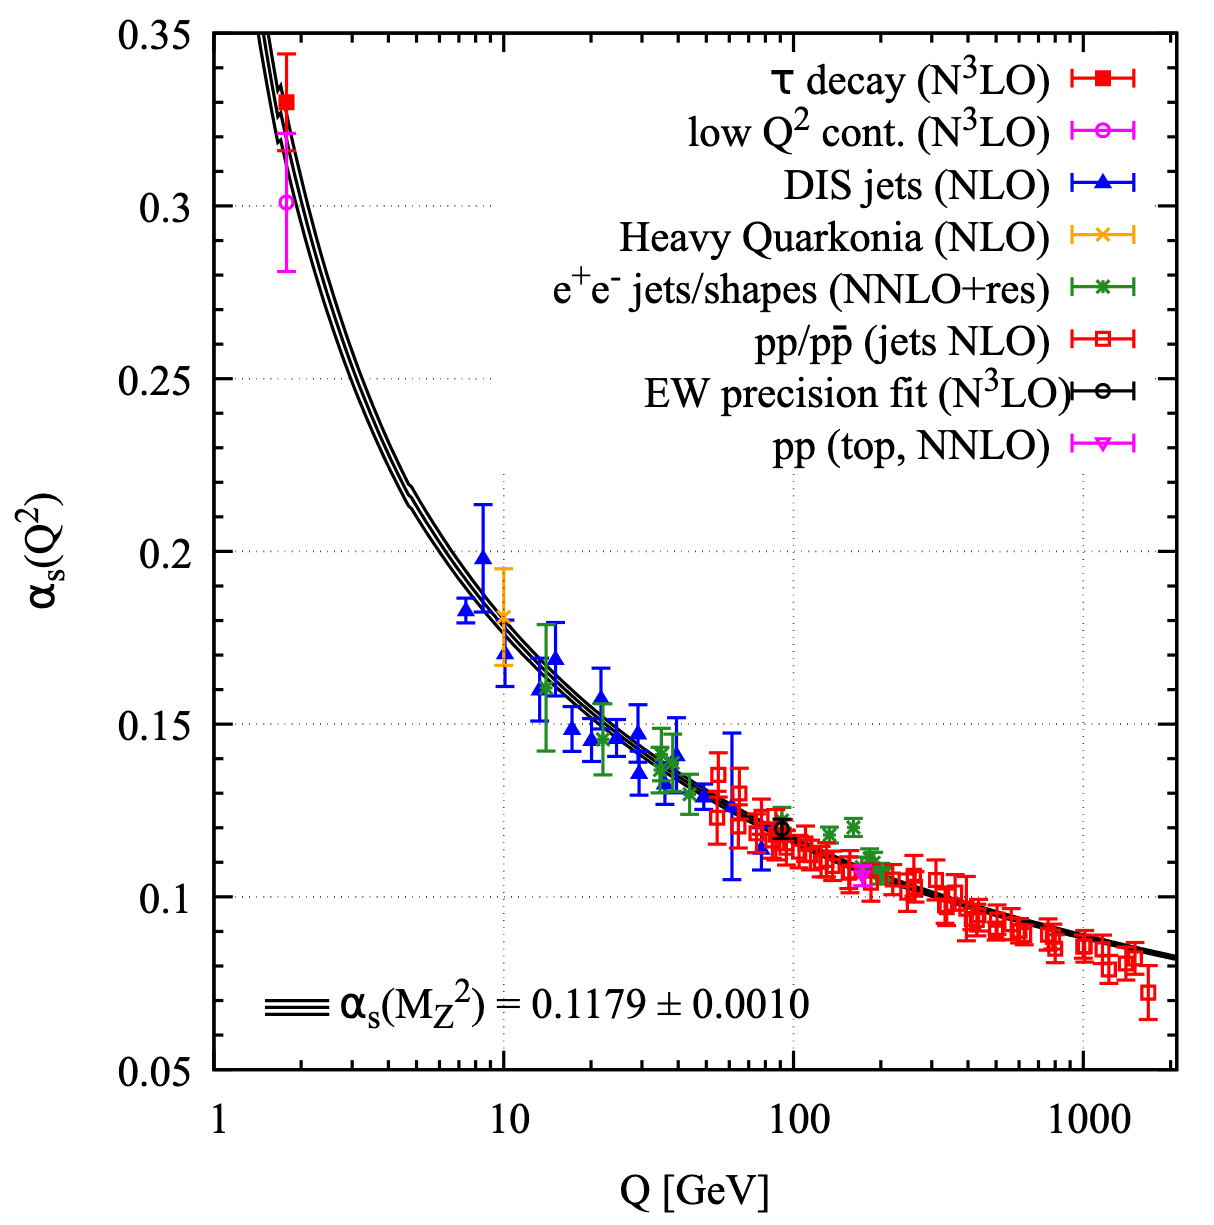
\includegraphics[width=0.75\textwidth]{alpha_s_measurements}
	\caption{
	Summary of measurements of the strong coupling $\alpha_s$ as a function of the energy scale $Q$.
	The respective order of QCD perturbation theory used in the extraction of $\alpha_s$ is indicated in parentheses.
	\cite{PDG:PhysRevD.98.030001}
	}
	\label{fig:alpha_s_measurements}
\end{figure}

This result shows that $\alpha_s$ \textit{decreases} as the interaction scale increases, in stark contrast to the other interactions of the SM.
Thus in the very high energy regime, QCD interactions become weaker, a phenomenon known as \textbf{asymptotic freedom}.
The inverse phenomenon, strong coupling in the low-energy regime, is known as \textbf{confinement}.
This unique property of QCD is responsible for \textbf{fragmentation}, the process by which high energy \textbf{partons} (quarks/gluons) split into a shower of additional partons and \textbf{hadronization}, the process by which this parton shower recombines into colorless hadrons at lower energy.
These effects make theory/computational efforts particularly difficult in QCD.

\subsection{Higgs Mechanism}
So far there are no mass terms, such as $-m_\Psi^2 \Psi^2$ for the fermions, in $\mathcal{L}_{\mathrm{EW}}$ or $\mathcal{L}_{\mathrm{QCD}}$.
In all cases these terms would break local gauge invariance if no other changes were made.
The solution to this problem is the inclusion of a complex-valued scalar\footnote{Scalar here means the field transforms as a scalar under Poincar\'{e} transformations. This is distinctly different than the left-handed fermions, though they are also $SU(2)$ doublets but transform as spinors.} field in an $SU(2)$ doublet representation.
\begin{align}
    \mathcal{L}_{\mathrm{H}} &= \left|D_\mu \Phi\right|^2 - \mu^2 \Phi^\dag \Phi + \lambda \left(\Phi^\dag \Phi \right)^2 \\
    \Phi &= 
    \begin{pmatrix}
    \phi^+ \\
    \phi^0 \\
    \end{pmatrix}
\end{align}
where $D_\mu$ is the covariant derivative for the electroweak interaction as specified in Eq.~\ref{eq:ew_deriv}.
The last two terms in $\mathcal{L}_{\mathrm{H}}$ define the Higgs potential, restricted to this form by the requirement that any new terms added to the SM Lagrangian density be both renormalizeable and invariant under the local $SU(2) \otimes U(1)$ symmetry group.

For the vacuum to be stable $\lambda$ must be greater than zero. For the case where $\mu^2 > 0$ the scalar field $\Phi$ develops\footnote{It is important to note here that there is no mathematical motivation for the value of $\mu$ and the presence of this vacuum expectation value for the Higgs field. This is a case where the Lagrangian is constrained by experimental observations rather than mathematical constraints.} a non-zero \textbf{vacuum expectation value} $\langle \Phi \rangle$.
Since the potential only depends on $\Phi^\dag \Phi$ there are an infinite number of degenerate states with minimum energy $\frac{\nu^2}{2}$ corresponding to this energy state.
Due to the degeneracy and $SU(2)$ gauge invariance we can freely choose to write $\langle \Phi \rangle$ in a convenient form:
\begin{equation}
\langle \Phi \rangle = \frac{1}{\sqrt{2}} 
    \begin{pmatrix}
    0 \\
    \nu \\
    \end{pmatrix}
\end{equation}
and then by expanding around this minimum the Higgs field can be written as
\begin{equation}
\Phi(x) = \frac{1}{\sqrt{2}} 
    \begin{pmatrix}
    0 \\
    \nu  + h(x) \\
    \end{pmatrix}.
\end{equation}

This way of encoding the Higgs field is called the \textit{unitary gauge}.
The remaining scalar field $h(x)$ is the massive, electrically neutral spin-0 Higgs boson. %TODO: cite
The usefulness of the unitary gauge is apparent when expanding the term from $\mathcal{L}_{\mathrm{H}}$ involving the covariant derivative:
\begin{align}
    \left|D_\mu \Phi\right|^2 &= \left| \left( \partial_\mu + i \frac{g'}{2} Y B_\mu + i \frac{g}{2} T_a W_\mu^a \right) h(x) \right|^2 \\
    &= \frac{\nu^2}{8} \left[
     g^2 \left\{ (W^1_\mu)^2 + (W_\mu^2)^2 \right\}^2 + (gW^3_\mu - g' B_\mu)^2
    \right].
\end{align}
At this stage one can define new fields as linear combinations of the previous $B_\mu$ and $W^a_\mu$ fields to simplify the above expression:
\begin{align}
    W_\mu^\pm &\equiv \frac{1}{\sqrt{2}} \left( W^1_\mu \mp i W^2_\mu \right) \\
    Z_\mu &\equiv \frac{1}{\sqrt{g^2 + g^{\prime 2}}} \left( g W^3_\mu - g' B_\mu \right) \\
    A_\mu &\equiv \frac{1}{\sqrt{g^2 + g^{\prime 2}}} \left( g' W^3_\mu + g B_\mu \right)
\end{align}
where each of these new fields now have familiar $\frac{m^2}{2}x^2$-type mass terms in the Lagrangian, leading specifically to masses of:
\begin{align}
    m_{W^\pm} &= \frac{g\nu}{2}, \\
    m_{Z} &= \frac{\nu}{2}\sqrt{g^2 + g^{\prime 2}}, \\
    m_{A} &= 0.
\end{align}

By choosing this gauge three of the four real scalar fields of $\Phi$ have disappeared, but they have re-emerged as components of the new $W$, $Z$, and $A$ fields which correspond to the Standard Model weak $W^\pm$/$Z$ bosons and the photon $A$.
This process just described by which the ground state of the Higgs field $\Phi$ breaks the $SU(2) \otimes U(1)$ gauge symmetry is called \textbf{spontaneous symmetry breaking}.

Even though the entire Lagrangian still retains $SU(2) \otimes U(1)$ symmetry, if re-written in terms of perturbations \textit{around} the asymmetric vacuum state, the Lagrangian re-organizes itself to represent a different set of particles.
Do not be mislead though, it is still the same Standard Model Lagrangian that describes the fundamental particle interactions (except gravity) both before and after spontaneous symmetry breaking, it is only the ``ground state'' of the universe that changes.
The general consensus is that the spontaneous breaking of the $SU(2) \otimes U(1)$ symmetry by the accumulation of $\langle \Phi \rangle$ is an event that actually occurred during the early moments following the big bang, specifically when the temperature dropped below $159.5 \pm 1.5$ GeV \cite{DOnofrio:2015gop}.

So far we have only shown how spontaneous symmetry breaking gives rise to the masses of the gauge bosons $W^\pm$, $Z$ and $A$.
In order to incorporate mass terms for the fermions, new terms must be added to the Lagrangian which involve the coupling of the Higgs field to the left \textit{and} right-handed fermions with a form proportional to $\bar{\Psi}_L h \Psi_R$.
The reason these new coupling terms must be added is simple: because they are \textit{possible} under all the contraints of Poincar\'{e} invariance, gauge invariance and renormalization, thus we cannot ignore them.
These new terms involve the \textbf{Yukawa coupling constants} $f_\Psi$ for each fermion, and after spontaneous symmetry breaking contribute fermion mass terms to the SM Lagrangian with the following form:
\begin{equation}
\mathcal{L}_{\mathrm{Yuk}} = \frac{f_\Psi \nu}{\sqrt{2}} \left( \bar{\Psi}_L \Psi_R + \bar{\Psi}_R \Psi_L \right)
\end{equation}
for each fermion $\Psi$ where $m_\Psi = \frac{f_\Psi \nu}{\sqrt{2}}$.

\section{Hadronic Collisions}
An accurate mathematical description of the physics processes in a $pp$ collision, such as the example outlined in Figure~\ref{fig:proton_collision_complications}, is extremely complicated.
For example, either of the incoming or outgoing partons may radiate to produce initial state radiation (ISR) or final state radiation (FSR).
These types of complications that arise are labelled as the \textbf{underlying event}, a generic term for the combined impact of colored beam remnants, additional $pp$ interactions from the same bunch crossing, ISR, FSR, pileup, noise, and more.
In most cases of interest to particle physics research, only particles coming from high-$p_T$ processes are studied and the underlying event serves in practice as a challenge to both experimental and theoretical methods.

\begin{figure}
	\centering
	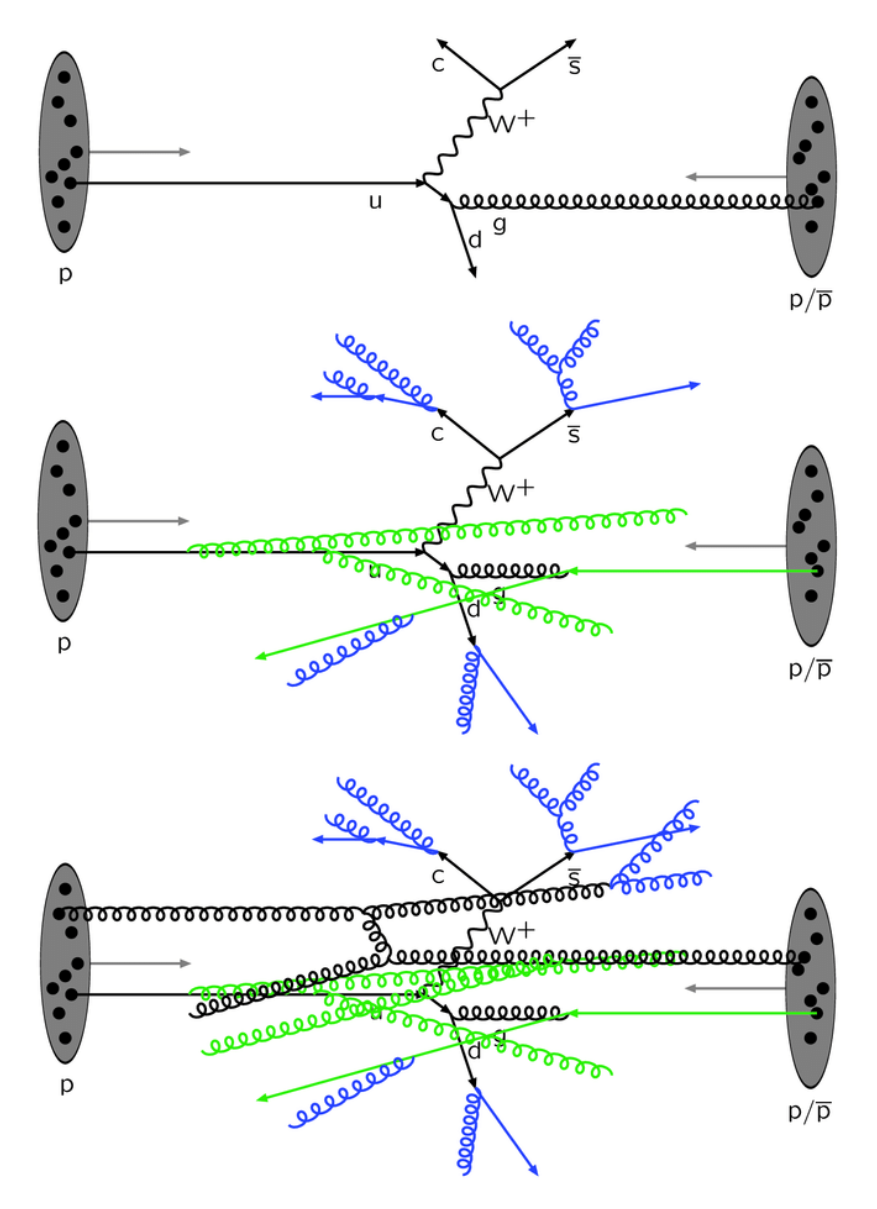
\includegraphics[width=0.75\textwidth]{proton_collision_complications}
	\caption{
	Sketch of a proton-proton collision at high energies with increasing levels of detail: (top) the hard scatter process only, (middle) including initial and final state radiation, and (bottom) inclusion of the underlying event, itself with additional initial and final state radiation \cite{Bechtel:2009zza}.
	}
	\label{fig:proton_collision_complications}
\end{figure}

The outgoing partons from the hard scatter event undergo \textbf{fragmentation} and \textbf{hadronization}, complex processes which involve different regimes of QCD which require different computation methods.
These processes of fragmentation and hadronization are a directly result of two fundamental properties of QCD discussed earlier: asymptotic freedom and confinement.
Luckily, the \textbf{factorization theorem} shows that the cross section for a scattering process between two partons $i$ and $j$ leading to the final state $X$ can be calculated by separating the high energy scale perturbative part of the interaction from the low energy scale non-perturbative part and treating them independently.

\begin{figure}
	\centering
	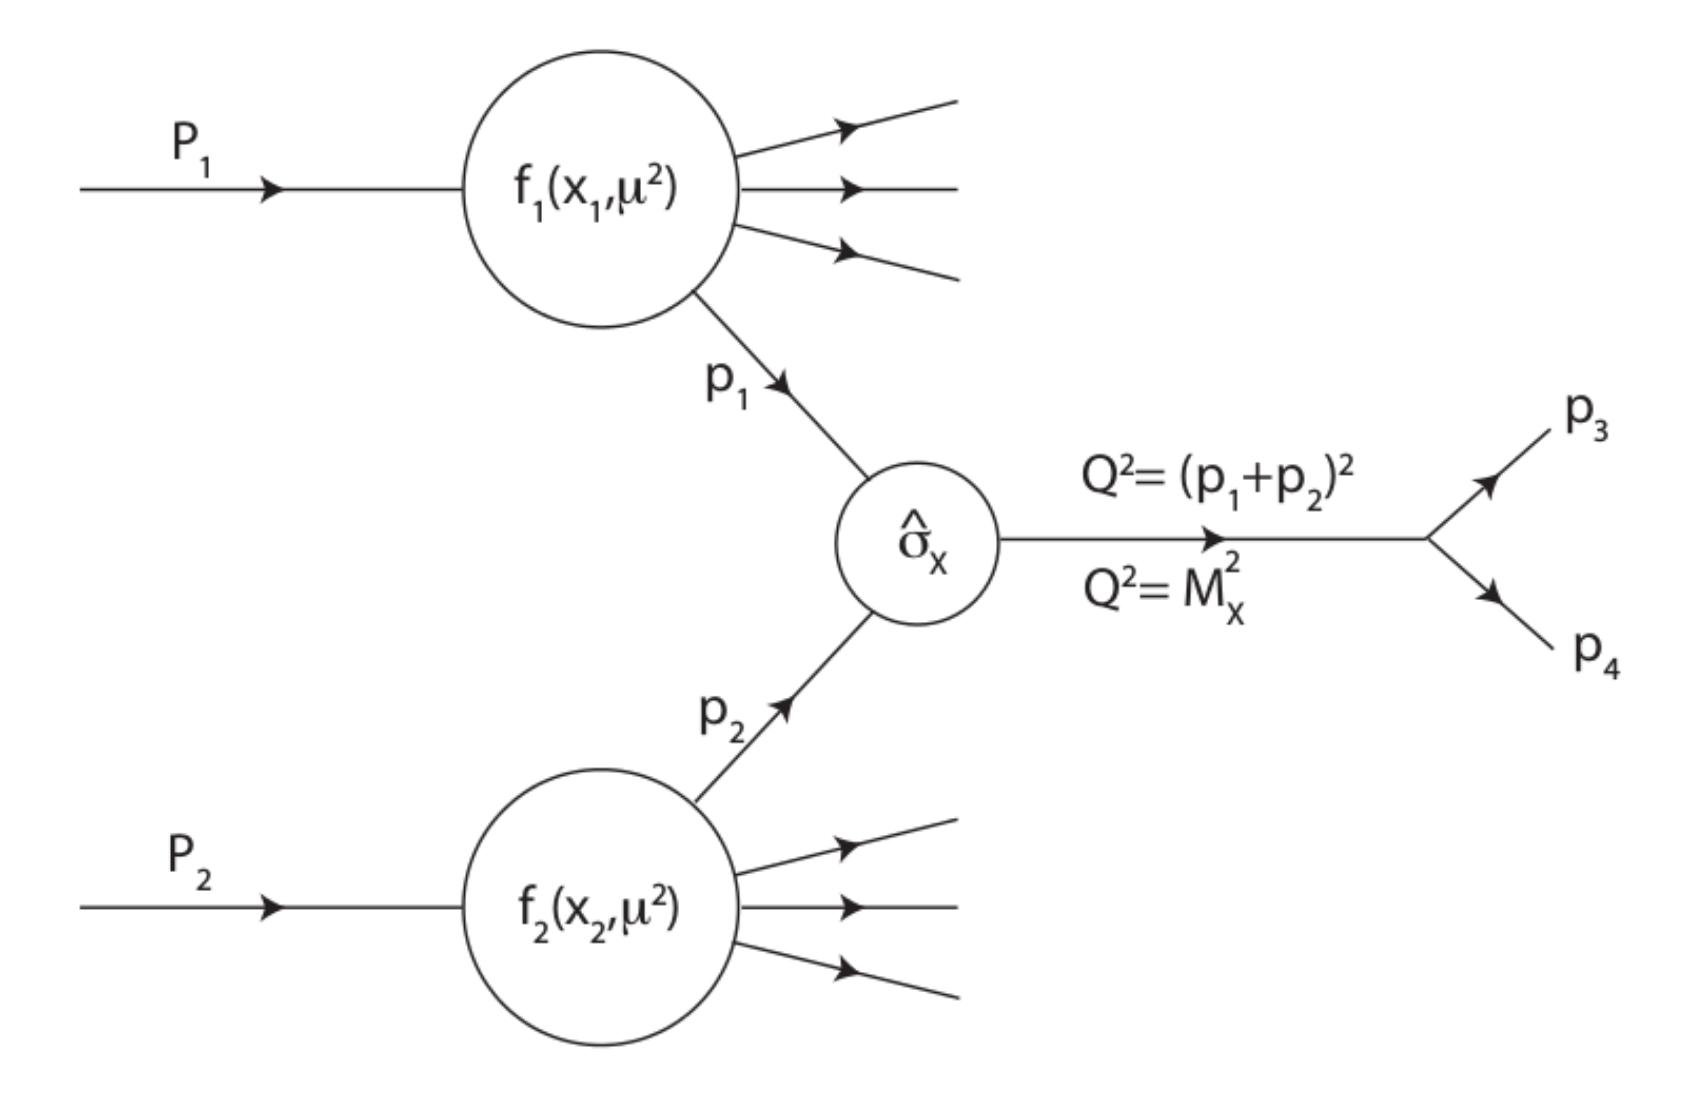
\includegraphics[width=0.75\textwidth]{factorization_diagram}
	\caption{
	Schematic diagram outlining the factorization theorem for the hard scattering of two protons with momentum $P_1$ and $P_2$.
	The parton distribution functions $f_i(x_i, \mu^2)$ give the probability to have a parton with a fraction $x_i$ of the proton momentum, and $\hat{\sigma}_x$ gives the cross section for the parton level interaction for two incoming partons with momentum $p_1$ and $p_2$. \cite{ellis_stirling_webber_1996}
	}
	\label{fig:factorization_diagram}
\end{figure}

What this means in practice is that the cross section for $pp \rightarrow X$ production can be computed using the cross section for the single parton-parton interaction of interest, weighting it with the probability for each parton to carry a given proportion of the proton momentum and integrating over all possible combinations of momentum fraction and initial state partons:
\begin{equation}
\sigma(P_1, P_2 \rightarrow X) = \sum_{i,j} \int \mathrm{d}x_1\; \mathrm{d}x_2\; f_i(x_1, \mu^2)\ f_j(x_2, \mu^2)\; \hat{\sigma}_{ij \rightarrow X}\left(p_1, p_2, \alpha_s(\mu^2), Q^2 / \mu^2 \right)
\end{equation}
where $P_1$ and $P_2$ are the four momenta of the incoming protons.
The four-momentum transferred between the partons during the hard scattering is $Q$.
The \textbf{parton distribution functions} $f_1$ and $f_2$ encode the probability for each initial state parton ($i$, $j$)\ to possess a certain fraction of the proton momentum $x_1$ and $x_2$ and they must be measured experimentally.
Thus the momentum of each parton can be written as  $p_1 = x_1 P_1$ and $p_2 = x_2 P_2$.
The factorization scale $\mu$ is a purely computational quantity resulting from \textit{renormalization}, an aspect of QFT required to make physical predictions particularly in the case of dealing with infinities that arise due to the effects of self interaction.
The cross section for $i,j \rightarrow X$ production is given by $\hat{\sigma}_{ij \rightarrow X}$, which depends on the strong coupling $\alpha_s$ and must take into account the factorization scale $\mu$ used in the PDF expressions.
A schematic of the factorization theorem is shown in Figure~\ref{fig:factorization_diagram}.

The total cross section is the sum of all cross sections for all possible $pp$ interactions that could be involved.
These interactions can be either elastic or inelastic.
Elastic collisions occur when both protons are preserved and no additional particles are produced.
Inelastic collisions result when at least one of the incoming protons is destroyed and the outgoing particles differ from the incoming particles.
Inelastic collisions are of predominant interest in particle physics as they probe fundamental interactions.

\section{Monte Carlo Simulation}
\label{sec:monte_carlo}
In order to interpret and understand experimental results from the ATLAS detector, comparisons to theoretical predictions must be made.
These predictions are often (but not always) necessary for predicting background rates, optimizing analysis selection, determining detector measurement resolution for various physical quantities, and more.
For collider physics, simulation involves not only the prediction of the underlying collision physics, but the interaction of the collision products with the detector itself.
In order to achieve this, the ATLAS experiment utilizes simulation based on Monte Carlo (MC) methods which rely on random sampling.

The ATLAS MC simulation proceeds in a serial manner where each step relies only on the output of the prior step.
An example illustration of a common $pp$ collision event outlining these steps is shown in Fig.~\ref{fig:pp_interaction}.
% TODO: find better figure here, it doesn't show hadronization...
These steps are (in order):
\begin{enumerate}
    \itemsep0em 
    \item Hard Scatter Event Generation
    \item Underlying Event Generation
    \item Parton Showering
    \item Hadronization
    \item Detector Simulation
\end{enumerate}

\begin{figure}
	\centering
	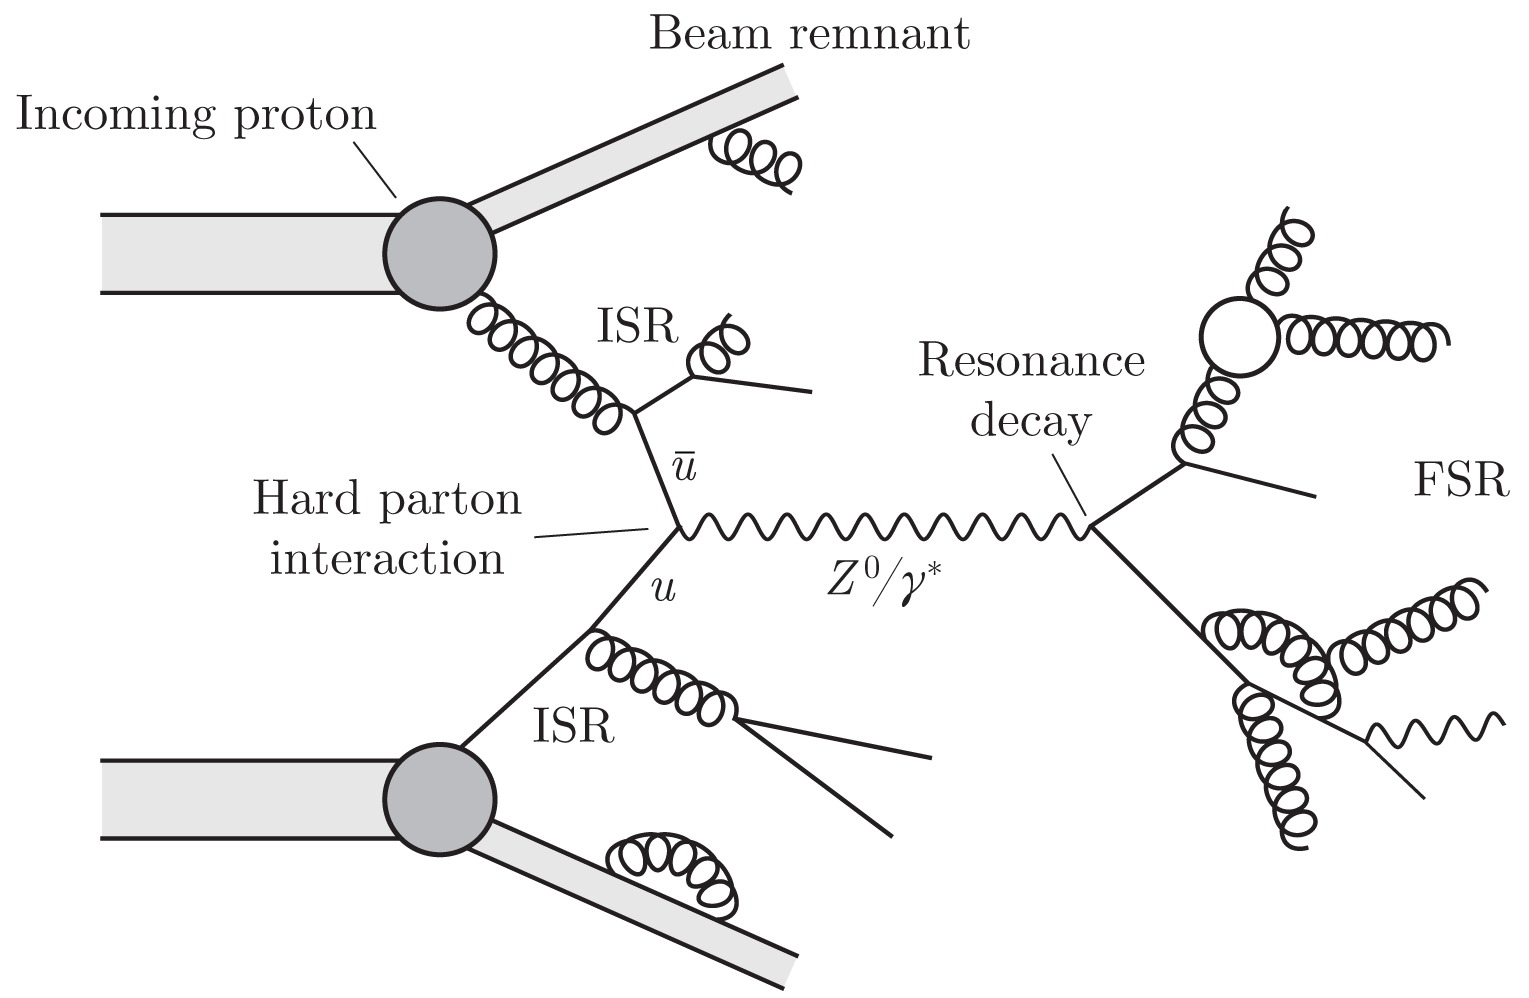
\includegraphics[width=0.75\textwidth]{pp_interaction}
	\caption{Illustration of an LHC proton-proton collision. © 2011 Chris Blanks}
	\label{fig:pp_interaction}
\end{figure}

\paragraph{\textbf{Hard Scatter Event Generation}}
Simulation begins with the hard-scatter process, or in other words, evaluation of a set of Feynman diagrams for some particular $2 \rightarrow n$ process.
In order to simulate collisions, parton distribution functions (PDF) must be used.
A parton refers to the strongly interacting particles (quarks and gluons) which protons are composed of.
These distribution functions describe the probability of finding a parton carrying a given fraction of the proton momentum.
These Feynman diagrams are used to compute the so-called \textit{Matrix Element} (ME) for the process via a perturbative expansion in powers of $(\alpha_s)$.
An intrinsic and unavoidable property of QCD known as ``asymptotic freedom'' asserts that this type of perturbative expansion is only valid at very high energies, or in other words, only for the immediate hard scatter event.
This breakdown occurs when the momentum scale of the collision products becomes $\approx 1$ GeV or less.
In this ``soft regime'' another simulation must pick up where the perturbative ME expansion left off.

\paragraph{\textbf{Underlying Event (UE)}}
In addition to the hard interaction generated, the interaction between the incoming proton remnants must be taken into account.
This is typically modelled through multiple $2 \rightarrow 2$ scattering processes occurring at a momentum scale of a few GeV.
The UE can include additional hard interactions and soft processes which cannot be computed perturbatively.

\paragraph{\textbf{Parton Showering}}
The ME method above works very well to describe hard parton interactions but is unable to correctly simulate the evolving collection of lower energy products that emerge from the products of the hard scatter.
In a manner similar to how accelerated electric charges radiate bremsstrahlung due to the rules of QED, colored partons emit QCD radiation in the form of gluons.
These radiated gluons can continue to radiate more gluons or split into quark-antiquark pairs.
This successive series of radiation/splitting results in a formation termed the ``parton shower'' which follows the evolution of the collision products momenta from the scale defined by the hard-scatter interaction down to the infrared scale at $\approx 1$ GeV at which point QCD becomes non-perturbative and confinement of the partons into hadrons takes place.

\paragraph{\textbf{Hadronization}}
As the shower approaches the QCD confinement scale $(\Lambda_{\mathrm{QCD}})$ the coupling forces become significant and the outgoing colored partons transform into colorless hadrons with a typical mass scale of $\approx 1$ GeV.
The hadronization process is also non-perturbative and relies on models which are tuned by experimental data, such as the Lund string model used by \Pythia and clustering models used by \Herwig and \Sherpa.

\paragraph{\textbf{Detector Simulation}}
To simulate the interaction of the simulated collision products with the ATLAS detector, the simulation results must be passed to a tool such as GEANT 4.
The detector simulation reproduces the effects of the particles passing through the various layers of the sub-detector components and relies on a detailed specification of the geometry, materials, and magnetic field inside the detector.
The physics processes involved in this detector simulation include ionization, bremsstrahlung, photon conversion, multiple scattering, scintillation, absorption, transition radiation, and more.
The last step in the simulation involves digitizing the output of the various detector components.
This is necessary to accurately reflect the raw data output of real events from the detector.
After digitization, simulated events may be fed to the reconstruction algorithms described in Chapter~\ref{ch:reconstruction} and processed exactly as if they were recorded data events.

